\documentclass[11pt, a4paper]{article}
\usepackage[UKenglish]{babel}
\usepackage[bibstyle=ieee, dashed=false, sorting=nty]{biblatex}
\usepackage[labelfont=bf]{caption}
\usepackage{csquotes}
\usepackage{fancyhdr}
\usepackage{float}
\usepackage{graphicx}
\usepackage[top=25mm, right=20mm, bottom=25mm, left=20mm]{geometry}
\usepackage[hidelinks]{hyperref}
\usepackage{microtype}
\usepackage{parskip}
\renewcommand{\baselinestretch}{0.4}
\usepackage[compact]{titlesec}

\titlespacing*{\section}{0pt}{\baselineskip}{0.35\baselineskip}

\pagestyle{fancy}
\fancyhf{}
\fancyhead[L]{COM3504}
\fancyhead[C]{The Intelligent Web: Assignment}
\fancyhead[R]{Team: Gakki}
\fancyfoot[C]{\thepage}

\addbibresource{references.bib}

\begin{document}
\section{Introduction}
Progressive Web App (PWA) allows users to create and add comments to both events and user stories. 
Social media features such as 'like', 'follow', 'interested', and 'going' are integrated. Users 
are able to tag an event along with their stories, which will then appear in the event page. Users 
can create a story by taking a picture with their front or environment camera through the 
implementation of WebRTC or upload a picture locally. Each user story can receive likes and comments, 
for which the latter is implemented using Socket.IO \cite{socketio, week6}. Service worker was 
implemented to cache requests for offline usage. MongoDB is used to store and synchronise data 
between the client and server, while IndexedDB is used to store data loaded from MongoDB for offline 
usage. However, data stored in MongoDB can only be retrieved when user is online. The search function 
(via location) was implemented with Google Maps API, allowing auto complete for the location field 
and ensuring that it is a valid location. For security purposes, users can only login with their 
respective Google Account.

\section{Diagrams}
\begin{figure}[H]
  \begin{center}
    \begin{minipage}[b]{0.4\textwidth}
      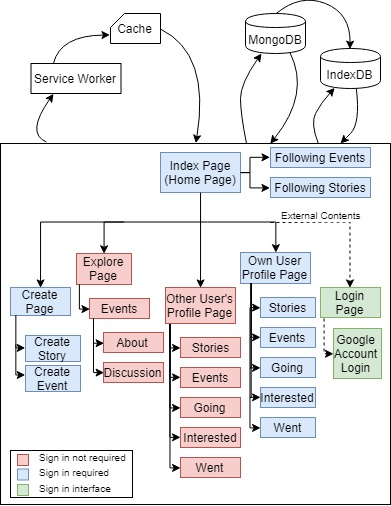
\includegraphics[width=6.5cm]{site_map.jpg}
      \caption{Demonstrates the flow of each web page in this PWA system along with the respective
      partial pages and external content pages.}
      \label{site_map}
    \end{minipage}
    %
    \qquad
    \begin{minipage}[b]{0.4\textwidth}
      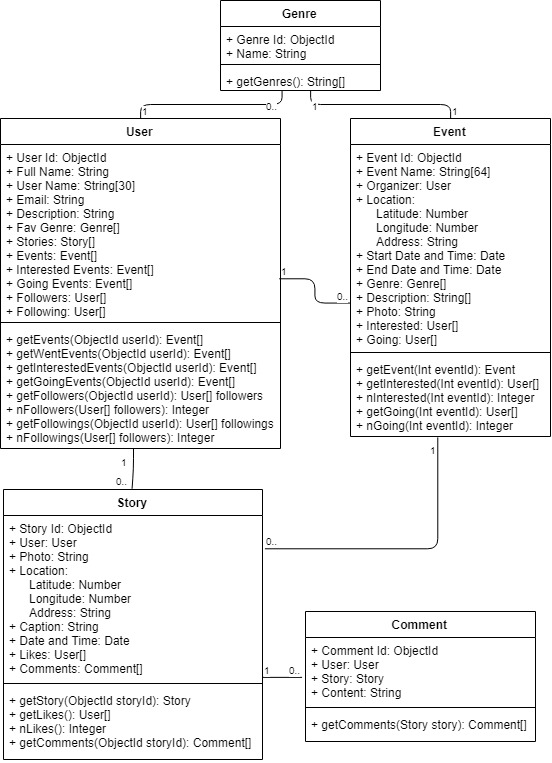
\includegraphics[width=6.5cm]{uml.jpg}
      \caption{Displays the structure of the database along with the types of content stored.}
      \label{uml}
    \end{minipage}
  \end{center}
\end{figure}
Figure~\ref{site_map} and figure~\ref{uml} are the detailed description of the PWA system structure
with figure~\ref{site_map} describing the front-end, data storage, caching and data retrieval, while
figure~\ref{uml} describe the types of data stored in the database along with the relationship
between documents.

\section{Interface to Insert and Search Data via Forms (Yet to Implement)}
\begin{itemize}
  \item \textbf{Challenges}: 
  \begin{itemize}
    \item Usage of search libraries which would allow suggestions and auto complete. 
    \item ElasticSearch only allow online searching and would cause errors when users are offline.
  \end{itemize}
  \item \textbf{Solution}: (Yet to Implement)
  \begin{itemize}
    \item Online library that would support offline searching so that users can make use of this 
    functionality both during online and offline.
  \end{itemize}
  \item \textbf{Requirements}: 
  \begin{itemize}
    \item Users should be able to search for events both during online and offline.
    \item Users should be able to search for events based on partial event names.
  \end{itemize}
%   \item \textbf{Limitations}: (Yet to Implement)
\end{itemize}

\section{Interface to Search Data via Map (Yet to Implement)}
\begin{itemize}
  \item \textbf{Challenges}:
  \begin{itemize}
    \item Implementation of Google API could not be cached, therefore could not be used offline. 
  \end{itemize}
%   \item \textbf{Solution}: (Yet to Implement)
  \item \textbf{Requirements}: 
  \begin{itemize}
    \item Allow users to search for events' location using map.
    \item Users should be able to use this search both offline and online.
  \end{itemize}
%   \item \textbf{Limitations}: (Yet to Implement)
\end{itemize}

\section{PWA – Caching of the App Template Using a Web Worker}
\begin{itemize}
  \item \textbf{Challenges}: 
  \begin{itemize}
    \item Image of events are not cached on initial load.
    \item Unable to cache user page through the use of service worker.
  \end{itemize}
  \item \textbf{Solution}:
  \begin{itemize}
    \item Alterations in service worker was conducted for imaged to load immediately and to cache 
    user profile data which is stored as $json$.
  \end{itemize}
  \item \textbf{Requirements}: 
  \begin{itemize}
    \item Users should be able to view a basic offline template with required data for when offline.
    \item Users should be able to view previously loaded events and stories without the ability to make 
    any changes to the events, stories, or their profiles.
  \end{itemize}
  \item \textbf{Limitations}: 
  \begin{itemize}
    \item Users are only able to view a basic offline template if no data were loaded in the past when 
    the user was online.
  \end{itemize}
\end{itemize}

\section{PWA: Caching Data Using IndexedDB}
\begin{itemize}
  \item \textbf{Challenges}:
  \begin{itemize}
    \item The usage of IndexedDB increases with every $put()$ operation.
  \end{itemize}
  \item \textbf{Solution}:
  \begin{itemize}
    \item There is no known solution at the moment, please refer to \cite{leveldb_593, leveldb_603} for 
    more information.
  \end{itemize}
  \item \textbf{Requirements}:
  \begin{itemize}
    \item Optimise IndexedDB to cache data to allow offline usage with limited data available.
    \item Users should be able to access essential data when offline for the application to serve its 
    purpose.
  \end{itemize}
  \item \textbf{Limitations}: 
  \begin{itemize}
    \item IndexedDB is stored locally and could not be updated until user is online.
    \item Disk Storage still increases with every $put()$ operation
  \end{itemize}
\end{itemize}

\section{NodeJS Server Including Non-Blocking Organisation of Multiple Dedicated Servers (Yet to Implement)}
\begin{itemize}
%   \item \textbf{Challenges}: (Yet to Implement)
%   \item \textbf{Solution}: (Yet to Implement)
  \item \textbf{Requirements}:
  \begin{itemize}
    \item The application should be able to connect to MongoDB server without explicitly starting MongoDB 
    server before starting the application. 
  \end{itemize}
%   \item \textbf{Limitations}: (Yet to Implement)
\end{itemize}

\section{MongoDB}
\begin{itemize}
  \item \textbf{Challenges}:
  \begin{itemize}
    \item Loading of initial data to populate the database.
    \item The retrieval and storage of images in the form of bits.
  \end{itemize}
  \item \textbf{Solution}:
  \begin{itemize}
    \item Initial population of database was resolved with the use of promises.
    \item Image retrieval and storage was implemented using $url$ format.
  \end{itemize}
  \item \textbf{Requirements}:
  \begin{itemize}
    \item Data stored in MongoDB is stored online. Data is not stored locally and cannot be
    retrieved offline. When user is online, data is retrieved from the database and displayed in 
    the PWA application.
  \end{itemize}
  \item \textbf{Limitations}:
  \begin{itemize}
    \item Initialisation of database needs to be run separately (refer to 'Extra Information').
    \item Data stored on MongoDB can only be accessed when user is online.
  \end{itemize}
\end{itemize}

\section{Quality of the Web Solution}
\begin{itemize}
  \item \textbf{Challenges}:
  \begin{itemize}
    \item Implementation of a secure login system.
  \end{itemize}
  \item \textbf{Solution}:
  \begin{itemize}
    \item Using Google Account to conduct login, at which users should use their existing Google 
    credentials to access the application.
  \end{itemize}
  \item \textbf{Requirements}:
  \begin{itemize}
    \item Users should be able to tag events in their stories, 'like' stories, 'follow' other 
    users, click 'interested' or 'going' on events.
    \item Events which users attended are recorded in their profile.
    \item Users require a Google Account to login for security purposes.
  \end{itemize}
  \item \textbf{Limitations}:
  \begin{itemize}
    \item Users without a Google Account could not use the system even though it is an unlikely case.
    \item User accounts are all public, hence users should be careful when sharing personal information.
  \end{itemize}
\end{itemize}

\section{Conclusions (To date of first submission)}
This assignment highlights the importance of caching and the importance of usability both during 
online and offline. It taught us to consider other implementations to improve user experience 
and web security. This assignment exposed us to multiple tools (like Google Maps API for 
address searching, WebRTC for photo capturing, etc.) while allowing us to implement the basic 
knowledge of web building at a higher level through the use of promises, service workers and memory 
caching.

\section{Division of Work (To date of first submission)}
The division of workload was lead by team leader, Eng Zer Jun. The solution was designed jointly 
and then each member lead the implementation of one specific part of the code. 
In particular:
\begin{itemize}
  \item \textbf{Eng Zer Jun}: lead the implementation of all PWA caching, MongoDB, and 
  front-end implementation
  \item \textbf{Lim Jia Mei Grace}: lead the report documentation, implementation of WebRTC, assisted 
  in the construction of MongoDB database and front-end implementation.
\end{itemize}

\section{Extra Information}
\begin{itemize}
  \item \textbf{System initialisation}: run 'npm install' prior to all of the following.
  \item \textbf{Connect to MongoDB}: (temporary) run 'mongod' to start serving MongoDB.
  \item \textbf{Initial population of MongoDB}: run 'npm run initdb' to drop database and
  repopulate database with default data.
  \item \textbf{Running the program}: run 'npm start' to start serving localhost.
\end{itemize}

\printbibliography

\end{document}
